\documentclass[11pt,a4paper]{report}
\usepackage[utf8]{inputenc}
\usepackage{amsmath}
\usepackage{graphicx}
\usepackage{gensymb}
\usepackage{tikz}
\usepackage{pgfplots}
\usepackage{mathtools}
\usetikzlibrary{arrows,positioning}
\tikzset{
    %Define standard arrow tip
    >=stealth',
    % Define arrow style
    pil/.style={
           ->,
           thick,
           shorten <=2pt,
           shorten >=2pt,}
}
\usepackage{geometry}
\geometry{
    left=2cm,
    right=0.64cm,
    top=0.64cm,
    bottom=2cm
}
\usepackage{multicol}
\setlength{\columnsep}{1cm}
\graphicspath{ {images/} }

\begin{document}

\chapter{Semester 2 Examination 2013-2014\\CZ4034 Information Retrieval}

\begin{multicols*}{2}

\section{Question 1}

\noindent \textbf{Question 1a} \\

\noindent \textbf{(i)} Define ``Document frequency''

\noindent Answer: Document frequency is number of times a term occurs in a collection of documents. Rare term has low document frequency, and is more informative than frequent terms.\\

\noindent \textbf{(ii)} Explain why an inverted index includes document frequencies.

\noindent Answer: In boolean retrieval, we retrieve results by performing boolean operation on posting lists. By knowing the document frequency, we can optimise boolean queries by processing AND operation in order of increasing document frequency.\\

\noindent \textbf{(iii)} Recommend the most plausible processing order for the Boolean query ``(blue OR sky) AND (red OR apple) AND (yellow OR pages)'', based on the following document frequencies:

\begin{center}
\begin{tabular}{ | l | l |} 
    \hline
    Term  & Document Frequency\\
    \hline
    blue  & 32874 \\
    sky   & 234 \\
    red   & 25143 \\
    apple & 324 \\
    yellow& 64563 \\
    pages & 463 \\
    \hline
\end{tabular}
\end{center}

\noindent Answer: Maximum number of document for:
\begin{itemize}
    \item (blue OR sky) = 33108
    \item (red OR apple) = 25467
    \item (yellow OR pages) = 65026
\end{itemize}

\noindent We do AND operation for (red OR apple) and (blue OR sky) first, then do AND operation for (yellow OR pages)\\

\noindent \textbf{Question 1b} Explain why IR systems typically do not remove stop words from their indexes. 

\noindent Answer: By having good compression techniques, the spaces that are required to store stop words are very small. In addition, by having good query optimization techniques, we only need to pay a little performance trade-off to include stop words. Furthermore, we need stop words for phrase query (e.g. King of Denmark) and relational query (e.g. flight to London). \\

\noindent \textbf{Question 1c} Compute the edit distance between ``SCE'' and ``CEE'' by using the dynamic programming algorithm of Levenshtein distance. 

\begin{center}
\begin{tabular}{ | l | l  l  l  l  |} 
    \hline
      &   & C & E & E \\
    \hline
      & 0 & 1 & 2 & 3 \\
    S & 1 & 1 & 2 & 3 \\
    C & 2 & 1 & 2 & 3 \\
    E & 3 & 2 & 1 & \textbf{2} \\
    \hline
\end{tabular}
\end{center}

\noindent \textbf{Question 1d} Give an instantiation of MapReduce function schema for bi-word index construction. Use an example to illustrate your answer.

\noindent Not in syllabus\\

\noindent \textbf{Question 1e} In a large collection of 100,000,000,000 Web pages, you find that there are 5,000 distinct terms in the first 10,000 tokens and 50,000 distinct terms in the first 1,000,000 tokens. If each Web page has 1,000 tokens on average, what is the size of the vocabulary of the index for this collection as predicted by Heap's law?

$$M=kT^b$$
$$5000=k(10000)^b$$
$$50000=k(1000000)^b$$

\begin{equation*}
\begin{split}
    \frac{5000}{(10000)^b}1000000^b &= 50000 \\
    10^{-4b}\cdot 10^{6b} &= 10 \\
    10^{2b} &= 10\\
    b &= 0.5\\
    k &= 50
\end{split}
\end{equation*}

\noindent When $T=10^{11} \times 10^3$, $M=500 \times 10^6$

\section{Question 2}

\noindent \textbf{Question 2a} Explain the following concepts with examples:\\

\noindent \textbf{(i)} Length normalization: A vector can be normalized by dividing each of its components by its length. Dividing a vector by its $L_2$ norm makes it a unit vector. Long and short documents now have comparable weights. Let say we have a document vector $\vec{d} = [1,1,0]$. We normalize the vector by using the following formula:

$$\vec{d}_{\text{norm}} = \frac{\vec{d}}{|\vec{d}|}$$

\noindent $|\vec{d}| = \sqrt{2}$, hence $\vec{d}_{\text{norm}} = [0.707, 0.707, 0]$ \\

\noindent \textbf{(ii)} Lossy compression: In lossy compression, the lost information after compression cannot be recovered. Several of the preprocessing steps can be viewed as lossy compression, such as case folding, stopwords, stemming, number elimination. \\

\noindent \textbf{(iii)} XPath: (not in syllabus) XPath is a syntax for defining parts of an XML document. XPath uses path expressions to navigate in XML documents. \\

\noindent \textbf{Question 2b} Illustrate the dictionary with the following terms, which is compressed by the techniques of dictionary-as-a-string and front coding, where the block size is 4:
\begin{center}
\verb|abcd,abel,able,abolish,|
\verb|bore,bored,bores,boring|
\end{center}

\noindent Answer:

\noindent \verb|4abcd4abel4able7abolish4bor*e2|$\diamond$\verb|ed2|$\diamond$\verb|es3|$\diamond$\verb|ing|
\noindent \verb|a                      b|

\begin{center}
\begin{tabular}{ | l | l | l |} 
    \hline
    Frequency & Posting pointer & Term pointer \\
    \hline
    1 & & a \\
    1 & & \\
    1 & & \\
    1 & & \\
    1 & & b \\
    1 & & \\
    1 & & \\
    1 & & \\
    \hline
\end{tabular}
\end{center}

\noindent \textbf{Question 2c} Give BOTH Variable Byte codes and Gamma codes for the following numbers: (i) 130 (ii) 45

\noindent Not in syllabus\\

\noindent \textbf{Question 2d} Consider the following collection of documents:
\begin{center}
Doc1: \verb|my love love star|\\
Doc2: \verb|I love star much|\\
Doc3: \verb|my star is your star|
\end{center}

\noindent Calculate the cosine similarity between documents in the collection, based on TF-IDF weighting, and select the closest pair.

\noindent Answer: before TF-IDF
\begin{center}
\begin{tabular}{ | l | l l l |l|} 
    \hline
    Term   & Doc1 & Doc2 & Doc3 & df \\
    \hline
    I      & 0    & 1    & 0    & 1  \\
    is     & 0    & 0    & 1    & 1  \\
    love   & 2    & 1    & 0    & 2  \\
    much   & 0    & 1    & 0    & 1  \\
    my     & 1    & 0    & 1    & 2  \\
    star   & 1    & 1    & 2    & 3  \\
    your   & 0    & 0    & 1    & 1  \\
    \hline
\end{tabular}
\end{center}

\noindent After TF-IDF:
\begin{center}
\begin{tabular}{ | l | l l l |l|} 
    \hline
    Term   & Doc1 & Doc2 & Doc3 & idf   \\
    \hline
    I      &0     &0.477 &0     & 0.477 \\
    is     &0     &0     &0.477 & 0.477 \\
    love   &0.229 &0.176 &0     & 0.176 \\
    much   &0     &0.477 &0     & 0.477 \\
    my     &0.176 &0     &0.176 & 0.176 \\
    star   &0     &0     &0     & 0     \\
    your   &0     &0     &0.477 & 0.477 \\
    \hline
\end{tabular}
\end{center}

\noindent After normalization:
\noindent After TF-IDF:
\begin{center}
\begin{tabular}{ | l | l l l |l|} 
    \hline
    Term   & Doc1 & Doc2 & Doc3 \\
    \hline
    I      &0     &0.684 &0     \\
    is     &0     &0     &0.684 \\
    love   &0.792 &0.253 &0     \\
    much   &0     &0.684 &0     \\
    my     &0.609 &0     &0.253 \\
    star   &0     &0     &0     \\
    your   &0     &0     &0.684 \\
    \hline
    length &0.289 &0.697 &0.697 \\
    \hline
\end{tabular}
\end{center}

$$\text{cosine}(\text{doc1},\text{doc2})=0.792 \times 0.253 = 0.200$$
$$\text{cosine}(\text{doc1},\text{doc3})=0.609 \times 0.253 = 0.154$$
$$\text{cosine}(\text{doc2},\text{doc3})=0$$

\noindent Doc1 and Doc2 are the closest

\section{Question 3}

\noindent \textbf{Question 3a} Consider a categorization task of classifying whether a user's review about a mobile app is informative (YES) or non-informative (NO). Table below shows a training set of 4 user reviews.

\begin{center}
\begin{tabular}{ | l | l |l|} 
    \hline
    ID & Words in user review & Informative? \\
    \hline
    1  & cool app fast excellent & NO \\
    2  & fast app drain battery & YES \\
    3  & cool fast crash bugs & YES \\
    4  & my favorite app bugs & YES \\
    \hline
\end{tabular}
\end{center}

\noindent \textbf{(i)} Based on the training set in the table, build a multinomial Naive Bayes classifier to classify the following user review:
\begin{center}\verb|fast cool bugs|\end{center}

\noindent Answer: There are 10 vocabulary:

$$P(NO) = \frac{1}{4}$$
$$P(YES) = \frac{3}{4}$$

$$P(\text{fast}|\text{YES}) = \frac{2 + 1}{12 + 10} = \frac{3}{22}$$
$$P(\text{fast}|\text{NO}) = \frac{1 + 1}{4 + 10} = \frac{2}{14}$$

$$P(\text{cool}|\text{YES}) = \frac{1 + 1}{12 + 10} = \frac{2}{22}$$
$$P(\text{cool}|\text{NO}) = \frac{1 + 1}{4 + 10} = \frac{2}{14}$$

$$P(\text{bugs}|\text{YES}) = \frac{2 + 1}{12 + 10} = \frac{3}{22}$$
$$P(\text{bugs}|\text{NO}) = \frac{0 + 1}{4 + 10} = \frac{1}{14}$$

\begin{equation*}
\begin{split}
P(\text{Yes}|\text{d}) &= \frac{\splitfrac{P(\text{fast}|\text{YES})P(\text{cool}|\text{YES})}{P(\text{bugs}|\text{YES})P(\text{YES})}}{P(\text{fast,cool,bugs})}\\
&= \frac{1}{P(\text{fast,cool,bugs})} \cdot \frac{3}{22} \cdot \frac{2}{22} \cdot \frac{3}{22} \cdot \frac{3}{4}\\
&= 0.00127k
\end{split}
\end{equation*}

\begin{equation*}
\begin{split}
P(\text{NO}|\text{d}) &= \frac{\splitfrac{P(\text{fast}|\text{NO})P(\text{cool}|\text{NO})}{P(\text{bugs}|\text{NO})P(\text{NO})}}{P(\text{fast,cool,bugs})}\\
&= \frac{1}{P(\text{fast,cool,bugs})} \cdot \frac{2}{14} \cdot \frac{2}{14} \cdot \frac{1}{14} \cdot \frac{1}{4}\\
&= 0.000364k
\end{split}
\end{equation*}

\noindent Since $P(\text{Yes}|\text{d}) > P(\text{NO}|\text{d})$, the user review is classify as informative (YES). 

\noindent \textbf{(ii)} Use the Rochhio classification algorithm with the training data in the table to classify the following review:
\begin{center}\verb|cool excellent my favorite|\end{center}

\noindent Answer: transform the table to vector space representation:

\begin{center}
\begin{tabular}{ | l | l l l l |} 
    \hline
    Term      & id1 & id2 & id3 & id4 \\ \hline
    app       & 1   & 1   & 0   & 1   \\
    bugs      & 0   & 0   & 1   & 1   \\
    battery   & 0   & 1   & 0   & 0   \\
    cool      & 1   & 0   & 1   & 0   \\
    crash     & 0   & 0   & 1   & 0   \\
    drain     & 0   & 1   & 0   & 0   \\
    excellent & 1   & 0   & 0   & 0   \\
    fast      & 1   & 1   & 1   & 0   \\
    favorite  & 0   & 0   & 0   & 1   \\
    my        & 0   & 0   & 0   & 1   \\
    \hline
\end{tabular}
\end{center}

\noindent We do a normalization without TF-IDF (you can do TF-IDF too). 

\begin{center}
\begin{tabular}{ | l | l l l l |} 
    \hline
    Term      & id1 & id2 & id3 & id4 \\ \hline
    app       & 0.5 & 0.5 & 0   & 0.5 \\
    bugs      & 0   & 0   & 0.5 & 0.5 \\
    battery   & 0   & 0.5 & 0   & 0   \\
    cool      & 0.5 & 0   & 0.5 & 0   \\
    crash     & 0   & 0   & 0.5 & 0   \\
    drain     & 0   & 0.5 & 0   & 0   \\
    excellent & 0.5 & 0   & 0   & 0   \\
    fast      & 0.5 & 0.5 & 0.5 & 0   \\
    favorite  & 0   & 0   & 0   & 0.5 \\
    my        & 0   & 0   & 0   & 0.5 \\
    \hline
\end{tabular}
\end{center}

$$\mu_{\text{NO}} = [0.5, 0, 0, 0.5, 0, 0, 0.5, 0.5, 0, 0]$$

\begin{equation*}
\begin{split}
\mu_{\text{YES}} &= [0.33, 0.33, 0.17, 0.17, 0.17, \\
&\ \ \ \ 0.17, 0, 0.33, 0.17, 0.17]
\end{split}
\end{equation*}

$$d_{\text{test}} = [0,0,0,0.5,0,0,0.5,0,0.5,0.5]$$

$$\text{cosine}(\mu_{\text{NO}}, d_{\text{test}}) = 0.5$$
$$\text{cosine}(\mu_{\text{YES}}, d_{\text{test}}) = 0.255$$

\noindent Since $\text{cosine}(\mu_{\text{NO}}, d_{\text{test}}) > \text{cosine}(\mu_{\text{YES}}, d_{\text{test}})$, we conclude that the review is not informative (NO). \\

\noindent \textbf{Question 3b} Let $|D|$ be the number of documents in training set, $|V|$ be the vocabulary size, and $|C|$ be the number of classes. Give the training time complexity of Naive Bayes algorithm, and indicate which term is expected to dominate the time complexity for most text collection.

\noindent Answer: the time complexity is $O(|C||V|+|D|)$. The term $|D|$ is expected to dominate the time complexity for most text collections. \\

\noindent \textbf{Question 3c} Briefly compare the bias-variance tradeoff between k-Nearest Neighbors and Naive Bayes algorithms

\noindent Answer: kNN has high variance and low bias. NB has low variance and high bias.\\

\noindent \textbf{Question 3d} In a university, first year students were given choice of studying a language subject of either French or Japanese. The numbers of male and female students choosing each language subject are shown in table below. Use the Chi-Square test at significance level $p=0.05$ (the critical value = 3.84) to test whether the choice of language is independent of sex.

\scriptsize
\begin{center}
\begin{tabular}{ |l|l|l|l| } 
    \hline
            & French     & Japanese   & Total \\
    \hline 
    Male    & $A = 39$   & $B = 16$   & $A+B=55$ \\
    Female  & $C = 21$   & $D = 14$   & $C+D=35$ \\
    Total   & $A+C = 60$ & $B+D = 30$ & $N=90$ \\
    \hline
\end{tabular}
\end{center}
\normalsize

\begin{equation*}
\begin{split}
   \chi^2(t,c) &= \frac{N\times (AD - BC)^2}{(A+B) \times (C+D) \times (A+C) \times (B+D)} \\
   &= \frac{90\times ((39 \times 14) - (16 \times 21))^2}{55\times 35 \times 60 \times 30}\\
   &= 1.145 < 3.84
\end{split}
\end{equation*}

\noindent With 95\% confident, we accept that the choice of language subject is independent of sex. 

\section{Question 4}

\noindent \textbf{Question 4a} Consider the 3-means clustering algorithm on a set $S$ consisting of the following 6 points in 2-dimensional space: $A=(0,0)$, $B=(8,0)$, $C=(16,0)$, $D=(0,6)$, $E=(8,6)$, $F=(16,6)$. The algorithm uses Euclidean distance metric to assign each point to its nearest centroidl ties are broken in favor of the centroid to the left/down. Assume that the tree initial centroids are based on data $A$, $C$, $D$, respectively. Perform the above 3-means clustering until it converges, and show the final clustering results.

\begin{tikzpicture}
\begin{axis}[
    enlargelimits=false,
    axis equal
]
\addplot+[
    nodes near coords,
    only marks,
    point meta=explicit symbolic
]
table[meta=label] {
    x y label
    0 0 A
    8 0 B
    16 0 C
    0 6 D
    8 6 E
    16 6 F
};
\end{axis}
\end{tikzpicture}

\noindent Answer: by looking at the plot, we know that point $B$ belongs to $A$, point $C$ belongs to $D$, and point $F$ belongs to $C$. Then, we update the centroids:

$$\mu_1 = [4,0]$$
$$\mu_2 = [16,3]$$
$$\mu_3 = [4,6]$$

\begin{tikzpicture}
\begin{axis}[
    enlargelimits=false,
    axis equal
]
\addplot+[
    nodes near coords,
    only marks,
    point meta=explicit symbolic
]
table[meta=label] {
    x y label
    0 0 A
    8 0 B
    16 0 C
    0 6 D
    8 6 E
    16 6 F
    4 0 $\mu_1$
    16 3 $\mu_2$
    4 6 $\mu_3$
};
\end{axis}
\end{tikzpicture}

\noindent After the first iteration, $A$ and $B$ in cluster 1, $C$ and D in cluster 2, and $D$ and $F$ in cluster 3. So, it converges.\\

\noindent \textbf{Question 4b} Considering a clustering task with a total of $N$ text documents. Design a clustering scheme which can output any desired number of cluster (1 to N) once the clustering task is completed. Brieftly discuss the time complexity of your clustering scheme. 

\noindent Answer: We can use agglomerative or divisive hierarchical clustering. Once the clustering task is completed, we can prune the hierarchical tree to achieve the number of cluster we want. The complexity of the algorithm is $O((N-1)(N^2))$ because we need $O(N^2)$ to update the proximity matrix, and we need to do it for $O(N-1)$ times. So, the complexity is $O(N^3)$.\\

\noindent \textbf{Question 4c} Consider a small web with 3 pages A, B, and C, where B links to A and C, while A links to C, and C links to A, as shown in the figure

\begin{center}
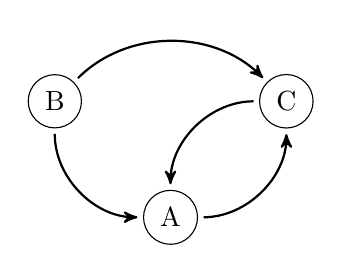
\begin{tikzpicture}[
roundnode/.style={circle, draw=black, thin},
]
%Nodes
\node[roundnode](A){A};
\node[above=of A](dummy){};

\node[roundnode](B)[left=of dummy]{B};

\node[roundnode](C)[right=of dummy]{C};

\path[pil] (B) edge [bend right=45] (A);
\path[pil] (C) edge [bend right=45] (A);
\path[pil] (A) edge [bend right=45] (C);
\path[pil] (B) edge [bend left=45] (C);

\end{tikzpicture}
\end{center}

\noindent \textbf{(i)} Compute the pagerank scores for each of the three pages. Assume that at each step of the pagerank random walk, we teleport to a random page with probability 0.09, with a uniform distribution over which particular page we teleport to

\noindent Answer: Transition matrix
\begin{center}
\begin{tabular}{ |l|l|l|l| } 
    \hline
      & A  & B  & C \\
    \hline 
    A & 0  & 0  & 1  \\
    B & 1  & 0  & 1  \\
    C & 1  & 0  & 0  \\
    \hline
\end{tabular}
\end{center}

\noindent Transition probability matrix
\begin{center}
\begin{tabular}{ |l|l|l|l| } 
    \hline
      & A    & B  & C \\
    \hline 
    A & 0    & 0  & 1  \\
    B & 0.5  & 0  & 0.5  \\
    C & 1    & 0  & 0  \\
    \hline
\end{tabular}
\end{center}

\noindent Transition probability matrix with teleporting
\begin{center}
\begin{tabular}{ |l|l|l|l| } 
    \hline
      & A    & B    & C      \\
    \hline 
    A & 0.03  & 0.03 & 0.94  \\
    B & 0.485 & 0.03 & 0.485 \\
    C & 0.94  & 0.03 & 0.03  \\
    \hline
\end{tabular}
\end{center}

$$x = [1/3,1/3,1/3]$$
$$xP = [0.485, 0.03, 0.384]$$
$$xP^2 = [0.485, 0.03, 0.384]$$

\noindent \textbf{(ii)} Compute the hubs and authorities scores for each of the three pages. In your solution, normalize the scores to ensure that the maximal hub score is 1 and maximal authority score is also 1.

\noindent Answer: first we initialize all hub and authority score to 1
\begin{center}
\begin{tabular}{ |l|l|l|l| } 
    \hline
         & A & B & C \\
    \hline 
    h(d) & 1 & 1 & 1 \\
    a(d) & 1 & 1 & 1 \\
    \hline
\end{tabular}
\end{center}

\noindent Compute the hub and authority score for each node
\begin{center}
\begin{tabular}{ |l|l|l|l| } 
    \hline
         & A & B & C \\
    \hline 
    h(d) & 1 & 2 & 1 \\
    a(d) & 2 & 0 & 2 \\
    \hline
\end{tabular}
\end{center}

\noindent Normalize
\begin{center}
\begin{tabular}{ |l|l|l|l| } 
    \hline
         & A     & B     & C \\
    \hline 
    h(d) & 0.408 & 0.816 & 0.408 \\
    a(d) & 0.707 & 0     & 0.707 \\
    \hline
\end{tabular}
\end{center}

\noindent Compute the hub and authority score for each node
\begin{center}
\begin{tabular}{ |l|l|l|l| } 
    \hline
         & A     & B     & C \\
    \hline 
    h(d) & 0.707 & 1.414 & 0.707 \\
    a(d) & 1.224 & 0     & 1.224 \\
    \hline
\end{tabular}
\end{center} 

\noindent Normalize
\begin{center}
\begin{tabular}{ |l|l|l|l| } 
    \hline
         & A     & B     & C \\
    \hline 
    h(d) & 0.408 & 0.816 & 0.408 \\
    a(d) & 0.707 & 0     & 0.707 \\
    \hline
\end{tabular}
\end{center} 

\noindent \textbf{Question 4d} Consider a scenario with two Web search engines A and B to estimate the frequency of duplicates on the Web. Each of the web search engines A and B crawls a random subset of the Web of the same size, respectively. Some of the pages crawled will be duplicates - exact textual copies of each other at different URLs. Assume that duplicates are distributed uniformly amongst the pages crawled by A and B. Further, we assume no pages have more than two copies; in other words, we will define a duplicate as a page that has exactly two copies. The search engine A indexes pages without duplicate elimination whereas the search engine B indexes only one copy of each duplicate page. Note that the two random subsets have the same size before duplicate elimination. If 45\% of A's indexed URL are present in B's index, while 50\% of B's indexed URLs are present in A's index, what fraction of Web consists of pages that do not have a duplicate?

\noindent Answer: we first find the size of B to A
$$A\cap B = \frac{45}{100}A = \frac{50}{100}B$$
$$\frac{B}{A} = \frac{9}{10}$$

\noindent However, the size of A and B are equal before duplicate elimination. So, there are $\frac{1}{10}$ of B indexes have been eliminated due to duplication. In conclusion, there are 90\% of the web consists of pages that do not have duplications.

\end{multicols*}
\end{document}
